\documentclass[accentcolor=tud2c,usenames,dvipsnames,colorbacktitle,inverttitle,landscape,german,presentation,t]{tudbeamer}
\usepackage[english]{babel}
\usepackage{amsmath}
\usepackage{amssymb}
\usepackage{color}
\usepackage{graphicx}
\usepackage{braket}
\usepackage[utf8]{inputenc}

\begin{document}

  \title{Exploring alternative SRG generators \\ in one dimension}
  % \subtitle{\small{Matthias Heinz, Kai Hebeler, Achim Schwenk}}
  \author{Matthias Heinz}
  \institute[Institut f\"ur Kernphysik, TU Darmstadt]{Institut f\"ur Kernphysik, TU Darmstadt}
  \date{March 18, 2019}

  \setbeamertemplate{section in toc}[ball unnumbered]
  \setbeamertemplate{subsection in toc}[ball unnumbered]


  \begin{titleframe}
    \begin{center}
      \textbf{\large{\underline{Matthias Heinz}, Kai Hebeler, Achim Schwenk}}\\
      \vskip1em
      \large{DPG Spring Meeting 2019, Munich} \\
      \vskip2em
      
\includegraphics[width=0.3\textwidth]{figures/01/logo_sfb1245}
    \end{center}
  \end{titleframe}

  \begin{frame}
    \frametitle{Potentials in Nuclear Physics}
    \begin{columns}[c]
      \begin{column}{0.6\textwidth}
        \begin{itemize}
          \item Finite-range attractive force
          \item Short-range repulsion
          \item Repulsion couples low and high momenta
          \item Leads to poor many-body convergence
        \end{itemize}
      \end{column}
      \begin{column}{0.4\textwidth}
        \begin{center}
          \includegraphics[width=\textwidth]{figures/02/hatsuda_phen-pot_new}
          \\ \footnotesize{Aoki et al., Comput.~Sci.~Dis.~(2008)}
          % cite https://iopscience.iop.org/article/10.1088/1749-4699/1/1/015009
        \end{center}
      \end{column}
    \end{columns}
  \end{frame}

  \begin{frame}
    \frametitle{The Similarity Renormalization Group (SRG)}
    \vskip-1em
    \begin{columns}[c]
      \begin{column}{0.5\textwidth}
        SRG:
        \begin{itemize}
          \item Class of continuous unitary transformations given by:
        \end{itemize}
        \begin{equation*}
          \frac{dH_s}{ds} = [[G, H_s], H_s]
        \end{equation*}
        \begin{itemize}
          \item $s=1/\lambda^4$
          \item $H_s$ goes to form of $G$
        \end{itemize}
        \vskip1em
        \visible<2->{Features:}
        \begin{itemize}
          \item<2-> Improved many-body convergence
          \item<2-> Induction of many-body forces
        \end{itemize}
      \end{column}
      \begin{column}{0.5\textwidth}
        \begin{center}
          \begin{overprint}
            \onslide<1>\includegraphics[width=0.82\textwidth]{figures/03/srg_potentials}
            \onslide<2>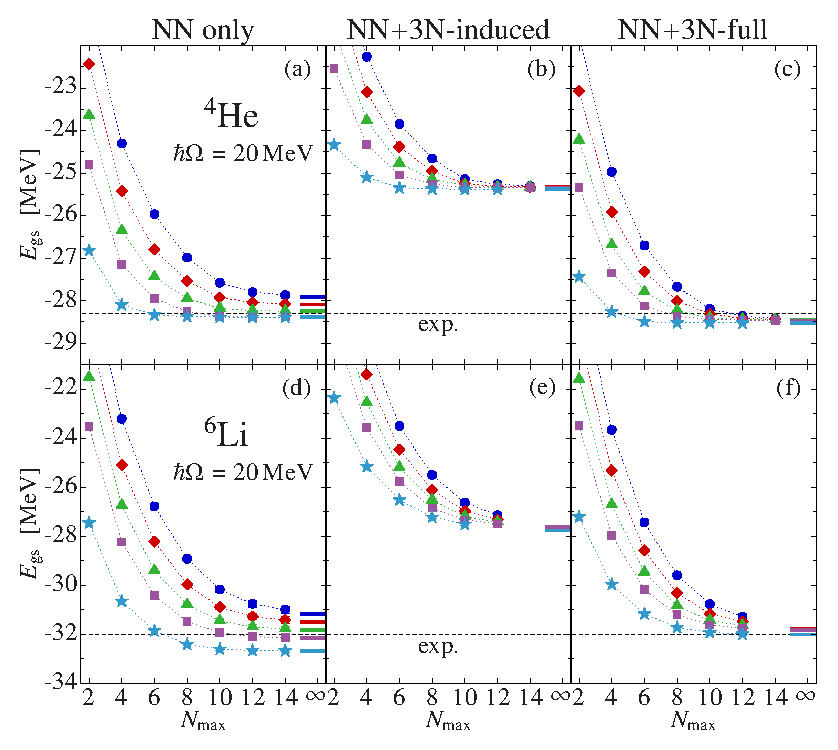
\includegraphics[width=\textwidth]{figures/03/roth1} \\
            \onslide<2>{\footnotesize{Roth et al., Phys.Rev.Lett.~107 (2011) 072501}}
            \onslide<3->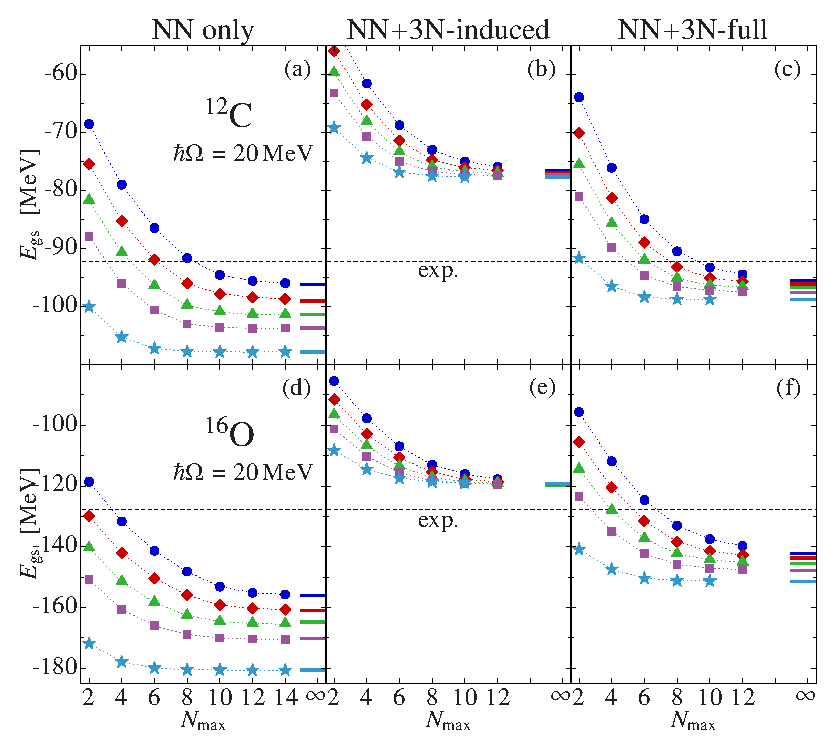
\includegraphics[width=\textwidth]{figures/03/roth2} \\
            \onslide<3->{\footnotesize{Roth et al., Phys.Rev.Lett.~107 (2011) 072501}}
          \end{overprint}
          % \visible<2->{\footnotesize{Roth et al., Phys.Rev.Lett.~107 (2011) 072501}}
        \end{center}
        % cite https://inspirehep.net/record/900106
      \end{column}
    \end{columns}
  \end{frame}

  \begin{frame}
    \frametitle{The Case for Alternative Generators}
    \begin{columns}[c]
      \begin{column}{0.9\textwidth}
        For $G = T_{rel}$:
        \begin{equation*}
          \color{black}\frac{dV_s(k, k')}{ds} = \textcolor{red}{-V_s(k, k')}(k^2 - k'^2)^2 + ...
        \end{equation*}
        \vskip-1.5em
        \begin{itemize}
          \item Exponential suppression for far off diagonal matrix elements
        \end{itemize}
        \vskip1em
        \pause
        For $G_s = T_{rel} + X_s$ with $X_s(k, k') = W(k, k') V_s(k, k')$:
        \begin{equation*}
          \color{black}\frac{dV_s(k, k')}{ds} = \textcolor{blue}{-(V_s(k, k') - X_s(k, k'))}(k^2 - k'^2)^2 + ...
        \end{equation*}
        \vskip-1.5em
        \begin{itemize}
          \item Change in matrix elements small when $X_s(k, k') = V_s(k, k')$
          \item Choose $W(k, k')$ to reflect what we want SRG to do
        \end{itemize}
      \end{column}
    \end{columns}
  \end{frame}

  \begin{frame}
    \frametitle{The ``Jurgenson'' Model \\ \normalfont \footnotesize{Jurgenson, Furnstahl, Nucl.Phys. A818 (2009)}}
    \vskip-2em
    \begin{columns}[c]
      \begin{column}{0.5\textwidth}
        Features:
        \begin{itemize}
          \item 1-D
          \item Bosons
          \item Negele potential
          \item Jacobi harmonic oscillator for many-body results
        \end{itemize}
        \vskip1em
        Advantages:
        \begin{itemize}
          \item Model is simple
          \item Results generalize well to 3-D calculations
        \end{itemize}
      \end{column}
      \begin{column}{0.5\textwidth}
        \vskip1.2em
        \includegraphics[width=\textwidth]{figures/05/negele_potential}
        % Missing figure of Negele potential
      \end{column}
    \end{columns}
  \end{frame}

  \begin{frame}
    \frametitle{Generator: $T_{rel}$}
    \begin{center}
      \vskip-2em
      \includegraphics[width=\textwidth]{figures/06/potentials} \\
      \includegraphics[width=0.30\textwidth]{figures/06/generator}
      \includegraphics[width=0.32\textwidth]{figures/06/decoupling}
      \includegraphics[width=0.32\textwidth]{figures/06/eigenvalues}
    \end{center}
    % \begin{equation*}
      % W(k, k') = 0
    % \end{equation*}
  \end{frame}

  \begin{frame}
    \frametitle{Generator: Block Diagonal}
    \begin{center}
      \vskip-2em
      \includegraphics[width=\textwidth]{figures/07/potentials} \\
      \includegraphics[width=0.30\textwidth]{figures/07/generator}
      \includegraphics[width=0.32\textwidth]{figures/07/decoupling}
      \includegraphics[width=0.32\textwidth]{figures/07/eigenvalues}
    \end{center}
    % \begin{equation*}
    %   W_{\Lambda,\epsilon}(k, k') = \frac{1}{exp(max(k, k') - \Lambda)/\epsilon^2) + 1}
    % \end{equation*}
  \end{frame}

  \begin{frame}
    \frametitle{Generator: Band Diagonal}
    \begin{center}
      \vskip-2em
      \includegraphics[width=\textwidth]{figures/08/potentials} \\
      \includegraphics[width=0.30\textwidth]{figures/08/generator}
      \includegraphics[width=0.32\textwidth]{figures/08/decoupling}
      \includegraphics[width=0.32\textwidth]{figures/08/eigenvalues}
    \end{center}
  \end{frame}

  \begin{frame}
    \frametitle{Outlook}
    \begin{columns}[c]
      \begin{column}{0.8\textwidth}
        Status:
        \begin{itemize}
          \item Have framework to test alternative generators
          \item Considering generators of form $T + WV_s$ \\ makes implementation of new generators easy
        \end{itemize}
        \vskip1em
        Direction:
        \begin{itemize}
          \item Incorporate 4- and 5-body binding energies
          \item Learn what features of generators lead to what behavior
          \item Identify features that lead to optimal results
        \end{itemize}
        \pause
        \vskip1em
        \begin{center}
          \large{Thank you!}
        \end{center}
      \end{column}
    \end{columns}
  \end{frame}



\end{document}
